\chapter{Results} % Main chapter title

\label{results} % For referencing the chapter elsewhere, use \ref{Chapter1} 

\lhead{Chapter 5. \emph{Results}} % This is for the header on each page - perhaps a 

\section{Full System Tests}
\label{sec:fullsystest}

An initial test of the completed system was performed using parameters similar to those in Figure \ref{fig:drvmatching}.  The complete conditions were as follows: 100,000 8-dimensional points were generated following the same procedure in Section \ref{sec:inittest}.  The ANN searches performed used a K of 20, and limited the number of nodes searched to 500.  This means that only about .5\% of the nodes were searched.  This test was performed using 80 different randomly generated DRVs, with 20 random points generated for each, again following the procedure in Section \ref{sec:inittest}.  This means that each index was tested against 1600 different queries.  The same MPDG error metric is also used, which measures the ratio of the average distance between the points in each query's result set and that of a linear search.  For our system, the default parameters described in Section \ref{sec:myimpl} were used.

Figure \ref{fig:fullsysrand} shows the MPDG performance of a standard k-d tree, out system, and that of a DRV matched k-d tree.  Both SMS and random split dimension selection heuristics were testsed.  From Figure \ref{fig:fullsysrand}, it is clear that the SMS based k-d trees tend to perform significantly better than those with random weights.  Thus, even though the offline construction cost of the random method is lower (due to not requiring a linear seek across each dimension), it is worth investing in WSMS, as this is is a one time cost and leads to significant improvement in result quality.  In fact, a single k-d tree using SMS had higher overall performance than our system when using SPM.  It is also important to note that the query DRVs used were pulled from a uniform distribution using the same method described in Section \ref{sec:inittest}.  As such, many of these DRVs were not drastically different from a standard uniform split.  Thus, while our data structure lead to a performance improvement for both splitting heuristics, the standard k-d tree still performed rather well.

\begin{figure}[h]
\begin{center}
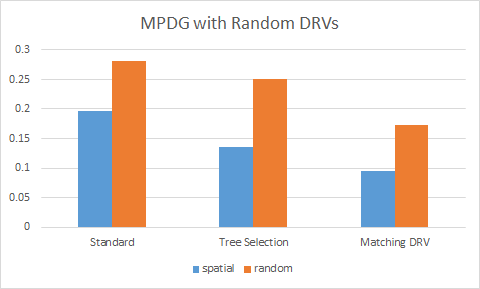
\includegraphics[width=.85\textwidth]{Figures/fullsysrand}
\end{center}
\caption{Full system test with random DRVs from uniform distribution}
\label{fig:fullsysrand}
\end{figure}

The real improvements came from extreme queries which only use a small subset of dimensions.  The same parameters for our system were chosen with the exception of setting the DDD to 3.  Following Equation \ref{eq:ddd}, 56 deterministic trees were used in addition to the 100 random trees and 1 tree generated from a uniform seed DRV.  The method of selecting the query DRVs was changed to only include a small subset of dimensions.  The method for doing so was to require at least a single dimension to be selected, and to determine whether or not other dimensions should be selected with a bernoulli random variable.  Thus, the distribution of the number of selected dimensions given a selection probability p and D dimensions is described by Binomial(D-1,p) + 1.  This test was run with p = .125.  After selecting a subset of dimensions, the weight of each dimension was drawn randomly from a uniform distribution and normalized to a sum of one.  Of note is that when only one dimension is selected it will have a weight of 1 in the DRV, and it would be ideal to only split on that dimension.  Fortunately, a seed DRV of all single dimension cases is included in our system, and as such there is guaranteed to be a tree which perfectly matches these DRVs and only splits on that single dimension.  In this case, the k-d tree performs equivalent to a binary search tree, and true nearest neighbors can be computed in O(log(N)) \citep{ahmadbinary}.  When more than one dimension is selected, while a perfect match tree likely won't exist (since weights are equal in seed DRVs), the two dimensional matching seed DRV will perform well if the query DRV is close to equal in the two dimensions, while the single dimension DRV will perform well when one dimension has a much larger weight than the other.  Additionally, k-d trees tend to be very effective with a low number of dimensions.

\begin{figure}[h]
\begin{center}
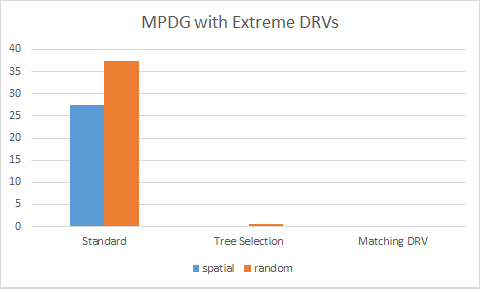
\includegraphics[width=.85\textwidth]{Figures/fullsysext}
\end{center}
\caption{Full system test with DRVs containing a low number of dimensions}
\label{fig:fullsysext}
\end{figure}

As shown in Figure \ref{fig:fullsysext}, with extreme queries our system's performance was extremely close to that of a single tree with a matched seed DRV, while the standard k-d tree performance suffered greatly.  The true performance of our system likely lies somewhere in the middle of the cases shown in Figures \ref{fig:fullsysrand} and \ref{fig:fullsysext}, as the true distribution of DRVs in seach queries is unknown.  Also of note is that seed DRVs with all sets of three dimensions were present, and close to 90\% of the selected DRVs had three or less dimensions.  However, even when four to five dimensions are selected performance is still expected to be strong, as the weights on a one or more of the dimensions will likely be low.

Because of the significantly stronger performance of WSMS compared to SPM, addtional tests have been performed only using the WSMS heuristic.  The key advantage to SPM is that all split dimensions are selected in constant time, wheras those in WSMS require a linear seek across all dimensions.  However, this cost is only associated with offline construction of the trees and is only performed once.  Since our benchmark attempts to optimize result quality on queries ignoring offline computation, WSMS is a superior heuristic according to our MPDG metric.  However, in Section \ref{sec:realworld}, we discuss that for a live system, it may be necessary to reconstruct trees on the fly, and therefore, when performance tuning, one should consider the merits of a heuristic with lower tree construction cost.

For our additional tests, three different indexes have been generated.  The first is a standard k-d tree for baseline performance.  The second is our system, using the standard parameters described above.  The final index generated is a single k-d tree using WSMS with a seed DRV matching that of the query DRV.  This case represents the hypothetical best case performance with our heuristics.

\section{Change of Dimensionality}

\begin{figure}[h]
\begin{center}
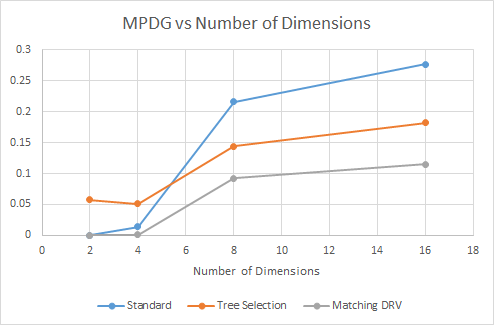
\includegraphics[width=.85\textwidth]{Figures/dims}
\end{center}
\caption{Full system test with data set of varying dimensions}
\label{fig:dim}
\end{figure}

It is important to consider how our system performs on data sets with different dimensionalities.  The data sets for these experiments have been generated following the procedure from \ref{sec:inittest}; however, the process has been replicated to generate data sets with different number of dimensions.  The results are shown in Figure \ref{fig:dim}.  For each index, the MPDG increases with dimensionality.  This is to be expected, as performance for k-d trees begins to degrade at higher dimensionalities.  Of note is that our system actually performed worse than a standard k-d tree for very low dimensionality.  This is likely because of the search time used to select the best trees.  Additionally, the k-d tree has the advantage of searching in a single tree, while searches in our index were split between multiple trees, and as seen in Figure \ref{fig:drvmatching} the performance of forests tends to be slightly worse than that of a single tree.  With a higher number of dimensions our system performs better than k-d trees, as the value of selecting trees with better seed DRVs is higher with more dimensions.  For 8 or more dimensions, performance is closer to the ideal case than the baseline.

\section{Size of Dataset}

We also tested the performance of our system on data sets of varying size.  Again the same procedure from \ref{sec:inittest} was followed, to generate datasets of dimensionality 8 with varying sizes.

\begin{figure}[h]
\begin{center}
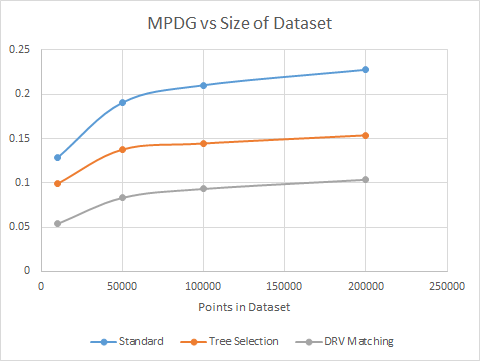
\includegraphics[width=.85\textwidth]{Figures/size}
\end{center}
\caption{Full system test with data set of varying size}
\label{fig:size}
\end{figure}

The results of this test are shown in Figure \ref{fig:size}.  For each of the indexes, the MPDG increases with the size of the dataset.  This is expected, searching a fixed number of nodes on a larger dataset means that a lower percentage of nodes are searched.  Of note is that the standard k-d tree index's performance decreased at a faster rate than that of our index and the tree with a matched seed DRV.  Thus, the benefits of our system are larger for bigger datasets. 

\section{Number of Trees}

The number of trees in our system is expected to have a direct impact on in its performance.  We tested our system against the same dataset described in \ref{sec:inittest}, generating our index with a varying number of random trees.

\begin{figure}[h]
\begin{center}
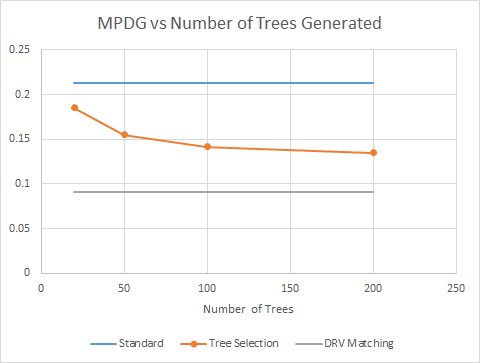
\includegraphics[width=.85\textwidth]{Figures/ntreesgen}
\end{center}
\caption{Full system test with varying number of random trees in our system}
\label{fig:ntreesgen}
\end{figure}

The results are shown in Figure \ref{fig:ntreesgen}.  The orange line represents the performance of the standard k-d tree, while the grey line represents the performance of a tree with a matched seed DRV.  With a larger number of trees, the overall quality of the selected trees will increase, since with more trees there are more chances for high quality matches.  However, this effect is diminishing.  As the number of trees increases, the performance gain from doing so drops.

\section{Nodes Searched}

\begin{figure}[h]
\begin{center}
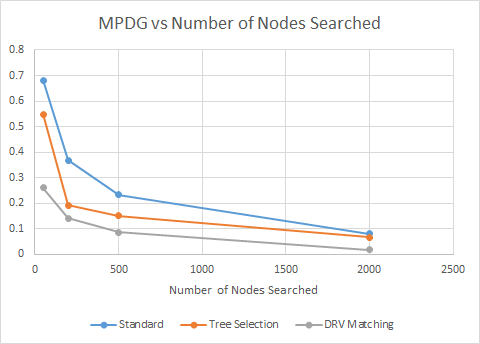
\includegraphics[width=.85\textwidth]{Figures/nsearch}
\end{center}
\caption{Full system test with varying number of nodes searched}
\label{fig:nsearch}
\end{figure}

We also considered the performance of our system for varying numbers of nodes searched.  The results for this test are shown in Figure \ref{fig:nsearch}.  As expected, for each index, the MPDG decreases with an increase in the number of nodes searched since a larger percentage of nodes are searched.  This effect is dimishing however.  Initially, an increase in the number of nodes searched leads to a large decrease in MPDG, wheras a similar increase when a large number of nodes are already searched has little effect.  Also of importance is that for a very small number of nodes searched our system's performance is close to that of a standard k-d tree.  This is because a high proportion of the alloted searches are used to select which trees to search.  As the number of searches increases so does our system's performance relative to the standard k-d tree.  Additionally, at a large enough number of searches, the standard k-d tree eventually catches up to our index as both converge to zero error.  Thus, our index was most effective when about .2\% to .5\% of the nodes were searched.

\section{Size of Result Set}

\begin{figure}[h]
\begin{center}
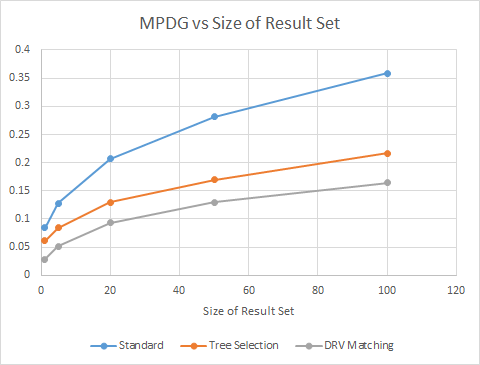
\includegraphics[width=.85\textwidth]{Figures/k}
\end{center}
\caption{Full system test with varying size of result set (K)}
\label{fig:kparam}
\end{figure}

The effect of the size of the result set (K) on MPDG was also tested.  Results are shown in Figure \ref{fig:kparam}.  For all indexes, the quality of the results decreased with larger K.  With a larger K, the index must find points with an increasingly large radius from the query point.  Since the ANN searches are performed most densely around the query point, the quality of further points is expected to be lower.  It should also be noted, that a because all branches must be searched which may contain a point closer than the current furthest point in the top K, with a larger K the stored furthest distance will be larger, and less branches of a tree can be pruned.  Of note is that with larger K, the quality of the standard k-d tree falls at a faster rate than that of our system.  This is because as the search expands outwards, since the split dimensions in our system are more optimal, closer points with the modified distance metric will be searched sooner, and more branches will be pruned allowing the search to expand deeper.

\section{Number of Trees Per Query}

\begin{figure}[h]
\begin{center}
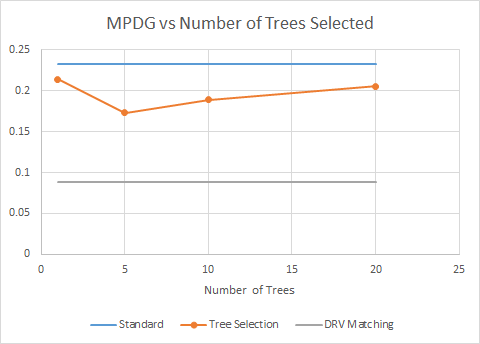
\includegraphics[width=.85\textwidth]{Figures/treesel}
\end{center}
\caption{Full system test with varying number of trees retrieved per query}
\label{fig:treesel}
\end{figure}

The number of trees searched per query (M) also has an effect on performance.  The results are shown in Figure \ref{fig:treesel}.  While with a perfect DRV match searching a single tree has the best performance, this is not the case when the DRV of a query does not perfectly match a tree's seed DRV.  Thus, when our system searches only one tree, because of the mismatch in these DRVs although performance is better than a standard k-d tree, it is not as high as when searching 5 trees in parallel.  When searching 5 trees, even though none of the trees are likely perfect matches, they add additional variety to the search, and likely introduce DRVs which are both too high and too low in each dimension rather than having a biased search.  However, increasing the number of trees too much prevents our system from searching as far in each tree and the performance begins to decrease.  Thus, the system should be tuned on this data set with around 5 trees.

\section{Alternative Dataset}

While it was demonstrated that our system consitently performs better than a standard k-d tree on the previous data set of uniformly distributed data, we also tested our system on a new data set with a drastically different distribution.  The data set selected was the Corel Image Features Color Histogram data set \citep{corelimage}. This data set of 68040 images has 32 dimensions, each of which represents the density of a range of colors in an image.  Similar images can then be computed based on these color densities from these 32 dimensional representations of the image.  It is important to note that this dataset was highly non uniform.  For most of the images a large number of the 32 dimensions had a value of 0 or close to zero.  Therefore, using the distance between the mininum and maximum elements is a poor metric of the length of a dimension.  Thus, our system was also benchmarked using the variance of a dimension as a measure of its spread during SMS.

\begin{figure}[h]
\begin{center}
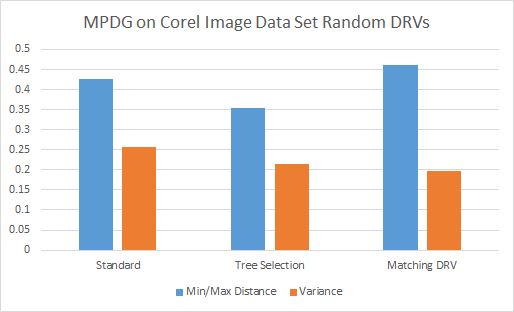
\includegraphics[width=.85\textwidth]{Figures/altrand}
\end{center}
\caption{Full system test on Corel Image Features Data Set with random DRVs from uniform distribution}
\label{fig:altrand}
\end{figure}

The results for the same search conditions as described in Section \ref{sec:fullsystest} are shown in Figure \ref{altrand}.  In this figure, all query DRVs were selected randomly with uniform weights on each dimension.  Interestingly, when using the poor maximum-minimum metric for SMS and WSMS, the tree with a perfectly matched DRV actually performed more poorly than our system.  This is likely because even though the seed and query DRVs matched, because of the flawed SMS dimension length metric poor split dimensions were selected.  When using variance however, performance is similar to that of our random dataset.  The performance of our system lies in between that of a standard k-d tree and a k-d tree with a matched seed DRV.

\begin{figure}[h]
\begin{center}
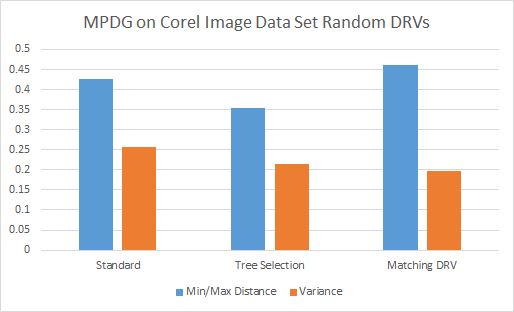
\includegraphics[width=.85\textwidth]{Figures/altext}
\end{center}
\caption{Full system test on Corel Image Features Data Set with DRVs with a low number of dimensions}
\label{fig:altext}
\end{figure}

This dataset was also tested with queries with a low number of dimensions shown in Figure \ref{fig:altext}.  The same procedure for generating seed DRVs from Section \ref{sec:fullsystest} was used; however, since this dataset had 32 dimensions instead of 8, p was set to .03.  Following a binomial distribution, this means that just under 80\% of the seed DRVs had 3 or less dimensions.  Additionally, because of the larger number of dimensions, DDD was set as 2 rather than 3.  With 100 random trees, and 1 additional tree with uniform seed DRV, our system used a total of 629 trees for this test.  Additionally, query points were pulled from the data set rather than generated randomly.  From Figure \ref{fig:altext}, it is clear that the trees generated with matching seed DRVs again have nearly zero MPDG.  This is because these trees only use a low number of dimensions, where k-d trees are most effective.  Our system's performance is still significantly better than that of the standard k-d tree, especially when using the variance for WSMS.  Because of the larger number of dimensions, we were restricted from setting the DDD to be larger, as increasing it to 3 would result in 4960 additional trees.  Thus, our index can be most effective on queries whose DRVs contain a low number of dimensions (or those with high weights on a small subset of dimensions) when the dimensionality of the data set is lower, as the DDD parameter can be increased with lower memory cost.